% 目次の挿入
\tableofcontents
\newpage

% ヘッダーカスタマイズ
\pagestyle{fancy}
\fancyhf{}
\fancyhead[L]{DLITE3:Technology that supports people's lives without boundaries}
\renewcommand{\headrulewidth}{0pt}
\makeatletter
\let\ps@plain\ps@fancy
\makeatother
% ヘッダーの下に空白を追加
\setlength{\headsep}{20pt}

\chapter{はじめに}
\section{背景}
 色覚障害は世界中で広く存在する問題であり、日本国内でも多くの人々が影響を受けている。一般的には、男性の約5\%、女性の約0.5\%が何らかの色覚異常を持っていると言われている。この割合を日本の人口に当てはめると、色覚障害を持つ人々の数はおよそ300万人以上に達している。色覚障害の影響は、日常生活や仕事の場面において多岐にわたり、特定の色を正しく認識できないことで困難が生じることが多々ある。例えば、交通信号や地図、データのグラフなど、色の識別が必要な状況では特に問題となる。これらの理由から、色覚障害に対する理解と支援が求められている。
\writer{佐々木工}

\section{色覚障害とは}
 色覚障害(色覚異常、色盲)は、通常の色を正確に認識することができない視覚的な障害だ。色覚障害の主な種類には以下のものがある:赤緑色覚異常(赤と緑の区別が難しい。これが最も一般的で、男性に多く見られる。P型(赤色盲): 赤色を感じることができない、または非常に弱い。D型(緑色盲): 緑色を感じることができない、または非常に弱い。)、青黄色覚異常(青と黄色の区別が難しい。これは非常に稀だ。T型(青色盲): 青色を感じることができない、または非常に弱い。)、A型(全盲色): すべての色を正しく感じることができない。非常に稀で、色を全く認識できない場合もある。色覚障害の多くは遺伝的な要因によるもので、染色体に関連している。また、怪我や病気、薬物の影響など後天的な要因でも色覚異常が発生することがある。色覚障害は、色覚検査(例: 石原式色覚検査)を使用して診断されている。色覚異常は日常生活に大きな影響を与えることも多く、特定の職業や活動で注意が必要な場合が多くある。
\writer{佐々木工}
\section{先行研究}
 \cite{色覚の多様性と色覚バリアフリーなプレゼンテーション}(細胞工学Vol.21 No.9 2002 p.1096~p.1099 岡部正隆 伊藤 啓)より、「●赤は,第1色盲の人に見やすいように朱赤にする. ●黄色と緑の間の黄緑系統の色は,赤緑色盲の人には黄色やオレンジと見分けがつかないのでぜんぶ避ける.●緑は赤や茶色と間違えないよう,青みの強いものを選ぶ.●紫は,青に近いと区別ができないので, なるべく赤に寄ったものを選ぶ.●朱赤から黄色の間では,見た目の明るさが違う3色(赤,オレンジ,黄色)を配分する.●青系では,見た目の明るさが違う水色と青を配分する.という基準で選んである.」と記載されている。このように色覚障害の種類によって配慮するべき点は異なる。\\
\cite{色のシミュレータ}は、様々な色覚特性を持つ人の色の見え方を体験するための伊木各シミュレーションツールである。スマートデバイスの内蔵カメラまたは画像ファイルから得た画像をリアルタイムに変換し、それぞれの色覚タイプ(2色覚)ではどのように色が見えるのか、シミュレーションを行う。\\
特徴\\
\begin{enumerate}
  \item 自身とは違う色覚を持つ人の世界をシミュレーションで体験することが可能。
  \item 1型(P型)、2型(D型)、3型(T型)の2色覚の色の見栄をリアルタイムに確認し、一般型(C型)の色の見えと比較することが可能。
  \item iPhone, iPad, iPodなどのiOSデバイス用、Androidデバイス用の両バージョンを提供しており、どこにでも持ち運び、いつでも色を確認することが可能。
  \item 色彩を大切に扱う分野で活動する人々におすすめである。
  \item 色彩学の理論に基づき、博士(医学・メディアデザイン学)である作者により開発された。
\end{enumerate}
\writer{小坂高義}

\section{研究動機}
 私たちは始め、視覚に障害のある方に向けたデバイスを考案しようとしていた。だが、考えていくうちに今社会に出回っているものを超えるものができるのかと考えたとき難しいと考えた。故にまずは視覚の中でも色覚に注目した。理由は班員の一人に色覚障害を持っている方がいて「肉を焼いてる時に色がわからない」「グラフや資料などの色がわからない時がある」という意見があった事が一つの理由だ。そういった点から色が見えないという色覚の悩みを解決できるデバイス、アプリケーションの開発を考えた。そのうえ色覚障害者は、日本だけでも300万人以上いる。故に、支援できるものが一つでも増えることが出来ればと考えた。
\writer{佐々木工}

\section{目的}
 色覚障害の人にとって見えない、見えにくいといったものは社会に出回っている。色覚障がい者向けの見えなかった資料、グラフなどの色が分かりやすくなることで今まで気づくこともできなかった問題が浮かびあがってくると考えた。色覚障がいは問題に気が付かないことが難しい点だ。見えないことを指摘して問題とすることは不可能でそれを解決する方法はない。故に私たちは見えないという問題が少しでも解決できるよう願って色を変換するアプリケーションを開発する必要があると感じた。
\writer{佐々木工}

\chapter{関連研究}
\section{必要なスキル}
 本プロジェクトにおいて重要なスキルの一つは、障害者の視点に立ち、そのニーズや困難を的確に把握する能力である。特に、対象者の日常生活や行動を観察し、彼らの立場に共感する力が求められる。加えて、対象者とのコミュニケーションを円滑に行い、適切な解決策を共に模索する姿勢が不可欠である。
\writer{水島知周}

\section{解決方法}
 課題解決の手法として、技術的な高度性よりも、簡便性および普及性を重視するアプローチが有効であると考えられる。特に、対象者に加えて支援者や家族といった幅広い利用者がストレスなく使用可能なツールを設計することが肝要である。このため、対象者の特性を踏まえつつ、汎用性の高い解決策を開発することが求められる。\\
\writer{水島知周}
\section{具体的な手法}
\subsection{ウェブアプリケーションの開発}
 本プロジェクトにおける具体的な解決手法として、ウェブアプリケーションの開発を提案する。ウェブアプリケーションは、プラットフォームに依存しない形で多様なデバイス上で利用可能であり、アクセシビリティの向上に寄与する。
特に、本プロジェクトでは以下の要素を重視して設計および開発を行う\\
\begin{enumerate}
  \item UI/UXデザインの最適化\\
  ユーザーにとって直感的で利用しやすいインターフェースを構築し、利用負荷を軽減する。\\
  \item アクセシビリティ基準への準拠\\
  WAI-ARIA(Web Accessibility Initiative - Accessible Rich Internet Applications)などの標準規格を活用し、視覚、聴覚、運動機能に制約を持つユーザーにも対応可能な設計を行う。\\
  \item レスポンシブデザインの採用\\
  パソコン、タブレット、スマートフォンなど多様なデバイスに適応するインターフェースを提供する。\\
  \item 多言語対応\\
  異なる文化圏や言語を使用する利用者のニーズを考慮し、グローバルな適用性を確保する。
\end{enumerate}
\writer{小坂高義}
\subsection{Pythonを活用したデータ処理と分析}
ウェブアプリケーションの基盤技術としてPythonを採用する。Pythonは、その簡潔で読みやすい文法と豊富なライブラリ群により、データ処理や分析の効率化を可能にする言語である。本プロジェクトにおいては、特に以下の分野でPythonを活用する\\
\begin{enumerate}
  \item データの前処理\\
  Pandasライブラリを使用して、障害者支援に関連するデータの整理やクレンジングを実施する。\\
  \item データ分析\\
  NumPyやScikit-learnを用いて、データの統計的解析や予測モデルの構築を行い、ユーザー行動に基づく適応的な提案機能を設計する。\\
  \item データ可視化\\
  MatplotlibやSeabornを活用し、解析結果を視覚化することで、利用者や関係者に直感的な理解を提供する。
\end{enumerate}
これらの技術は、「データサイエンス入門」という講義で学んだ内容を基礎としている。この講義では、Pythonを活用したデータ分析手法の基本概念から実践的な応用までを学び、その知見を本プロジェクトに応用した。これらの技術要素を統合的に活用することで、実用性およびユーザーへの有用性を兼ね備えたウェブアプリケーションを構築することを目指す。
\writer{水島知周}

\chapter{本プロジェクト学習の目標}
 本プロジェクトの最終的な学習目標は、色覚障害を持つ人々が日常生活や職場、教育現場において直面するさまざまな困難を軽減し、社会全体のバリアを取り除くことである。この目標を達成するために、1章および2章で明確にした課題と解決策を基盤として、具体的な成果物としての「色覚変換アプリケーション」の開発を行う。このアプリケーションは、色覚障害者が視覚的な情報をより正確かつ直感的に理解できるよう支援することを目的としており、情報格差の是正に向けた一歩を担うことを目指している。
\writer{佐々木工}
\section{色覚変換アプリケーションの完成}
 このアプリケーションの開発においては、以下の具体的な機能と特徴を盛り込むことを目指す。
\begin{enumerate}
  \item 視覚的情報の色変換機能の実装\\
  図表、グラフ、プレゼンテーション資料など、多くの場面で使用される視覚的情報の色を、色覚障害者が視認しやすい配色に変換する機能を実装する。これにより、職場や教育現場などでのコミュニケーションの円滑化が期待される。\\
  \item 画像やPDFデータの対応\\
  アプリケーションに画像やPDF形式のデータを読み込ませることで、直接的に色の変換を行う機能を搭載する。これにより、紙媒体やデジタル資料を問わず、色覚障害者にとって使いやすいソリューションを提供する。\\
  \item 代替テキストの添付機能\\
  色の変換だけでなく、資料の重要な情報をテキストで補足する「代替テキスト」機能を組み込むことで、情報のアクセシビリティをさらに向上させる。この機能は、視覚障害やその他の障害を持つ方々にも有益であり、より幅広いユーザー層への対応が可能となる。
\end{enumerate}
\section{水島知周}
\section{色覚バリアフリーの促進}
 開発したアプリケーションを通じて、色覚障害を持つ人々が抱える課題に対する社会的な認識を深め、より多くの人々にカラーユニバーサルデザイン(CUD)の重要性を伝えることを目指す。この取り組みは、以下のような具体的な社会的影響を期待している。
\begin{enumerate}
  \item 色覚障害者がこれまで難しいと感じていた特定の職業や教育環境での障壁を減少させることで、多様な人材が活躍できる社会を構築する。
  \item 色覚に配慮したデザインや情報提供の重要性を広めることで、行政機関や教育機関、企業などの取り組みを促進する。
\end{enumerate}
\writer{水島知周}
\section{実践的なスキルの習得}
 本プロジェクトの学びの一環として、次のような技術的および実践的なスキルの習得を目指す。
\begin{enumerate}
  \item OpenCVライブラリの活用\\
  OpenCVを用いて色変換アルゴリズムを実装し、色の識別における課題を解決するための技術を学ぶ。このアルゴリズムの実装は、精度だけでなく、処理速度や柔軟性の観点からも最適化を目指す。\\
  \item 課題解決能力とチームワークの向上\\
  プロジェクトを通じて、実社会での課題を解決する方法論を学び、チームでの協働作業の重要性を理解する。また、プロジェクトを計画し、実行する中で、実践的な応用力を磨く。
\end{enumerate}
\writer{佐々木工}
\section{最終的な目標と期待される成果}
 本プロジェクトの成果物である色覚変換アプリケーションが広く社会で活用されることで、色覚障害者が日常生活や職場、教育現場における情報をより正確に理解できるようになることを目指す。それによって、彼らが自信を持って活動できる環境を整えるだけでなく、多様性を尊重する社会の構築にも貢献することが期待される。また、本プロジェクトを通じて得た知識や経験を次の学びに活かし、社会課題の解決に積極的に取り組む開発者として成長することも目標として掲げている。これにより、プロジェクトの成果が単なる技術的な開発にとどまらず、広く社会的な影響を与えることが可能になると確信している。
\writer{水島知周}

\chapter{目的を達成するための手法・手段}
\section{アンケート}
 2024年10月31日から11月30日にかけて、色覚異常者を対象としたアンケートを実施した。本調査の目的は、色覚異常の詳細を明らかにすることとした。当初は未来大学の学生を対象としていたが、11月7日以降は未来大学以外の対象者も含めて回答者を募る方針とした。アンケートはGoogleフォームを用いたオンライン形式で実施した。
\section{北村翁}
\section{アイデアの概要}
 色覚障がい者が図やグラフの色を認識しやすくするために、スマートフォンを用いて画像を撮影し、色変換を行うアプリケーションを開発する。変換後の画像は、色覚障がい者にとって視認性が向上した状態で画面に表示される。また、画像内の重要な情報については代替テキストを自動的に生成し、ユーザーが視覚的情報をより深く理解できるようにする。
\section{水島知周}
\section{使用技術}
 今回のプロジェクトで開発したアプリケーションは、Pythonで実装した。画像ファイルを読み込み、OpenCVライブラリを使って各ピクセルの色情報を解析し、色覚障がい者が見やすい色に変換する技術を取り入れた。具体的には、NPO法人カラーユニバーサルデザイン機構(CUD)が提唱する色覚の多様性に対応したカラーユニバーサルデザインを活用し、解析した色情報をCUDに基づくカラーコードに上書きする手法を採用した。この手法によって、図やグラフなどで色の識別が難しい場合の視認性向上を目指した。
さらに、色覚の型ごとに視認性が悪い色の使用量を減らし、見えにくい色を避けて判別しやすい色だけを使う方法を採用した。また、色変換のアプローチを単一化した際に想定外の変換が起こる可能性を考慮して、以下の2つの方法を検討した。一つ目は、グレースケール化によってカラーのトーンだけを保存する方式。二つ目は、HSV形式で色を18段階に分け、範囲を指定して画像を強制的に18色に書き換える方式だ。
\writer{水島知周}

\subsection{Python}
 Pythonは、高レベルで汎用性のあるGuido van Rossum(グイド・ヴァン・ロッサム)氏が開発したプログラミング言語であり、シンプルで読みやすい構文を特徴としている。この言語は、ウェブ開発、データ解析、人工知能、機械学習、ゲーム開発、スクリプト作成など、さまざまな分野で広く利用されている。Pythonのコードは可読性が高く、初心者でも学びやすいことから、プログラミング教育の場でもよく使用されている。また、Pythonは豊富なライブラリとフレームワークを持ち、DjangoやFlaskを用いたウェブアプリケーション開発、NumPyやPandasを使ったデータ解析、TensorFlowやPyTorchを活用したAIモデルの構築など、専門的な分野にも対応している。さらに、オープンソースであり、Windows、macOS、Linuxといったさまざまなプラットフォームで動作するため、開発環境に依存しない柔軟性がある。Pythonを用いることで、効率的かつ多様なアプリケーションを開発することが可能である。
\writer{水島知周}
\subsection{HTML (HyperText Markup Language)}
 HTMLは、ウェブページを構築するための基本的なマークアップ言語であり、ウェブページの構造および内容を記述するために使用される。具体的には、テキスト、画像、リンク、フォーム、表などの要素を「タグ」を用いて定義することで、その内容を表現する。HTMLはインターネットにおける標準技術として位置付けられ、ウェブページ作成の基盤を提供するものである。また、CSS(Cascading Style Sheets)やJavaScriptと併用することで、スタイルの適用や動的な機能の追加が可能となる。これにより、ウェブページの設計およびユーザー体験を高度に制御することが可能となる。
\writer{小坂高義}
\subsection{CSS (Cascading Style Sheets)}
 CSSは、HTMLで記述されたウェブページの視覚的デザインおよびレイアウトを管理するためのスタイルシート言語である。HTMLがウェブページの「構造」を定義するのに対し、CSSはその「見た目」を制御し、フォントの色やサイズ、背景色、要素の配置、余白などを指定する役割を担う。CSSの使用により、コードの再利用性と管理効率が向上する。また、レスポンシブデザインの実現により、異なるデバイス(例: PCやスマートフォン)に適応したウェブデザインが可能である。このように、CSSはウェブページの視覚的品質を向上させ、ユーザー体験を強化する技術として重要な位置を占めている。
\writer{小坂高義}
\subsection{JavaScript}
 JavaScriptは、ウェブページに動的かつインタラクティブな機能を付加するためのプログラミング言語である。この言語を使用することで、HTMLやCSSでは実現が困難な機能を実装できる。具体的には、ユーザーの操作に応じたコンテンツの更新や、アニメーション効果の追加が可能である。また、JavaScriptはオペレーティングシステムやブラウザに依存せず、多くの環境で動作する汎用性を有している。主にクライアントサイドでのスクリプト言語として利用されるが、近年ではNode.jsを利用したサーバーサイド開発、さらにはデスクトップアプリやモバイルアプリ開発の分野にも広く応用されている。これにより、JavaScriptは現代のウェブ技術の中核を成す存在となっている。
\writer{小坂高義}
\subsection{PythonAnywhere}
 PythonAnywhereは、クラウドベースでのPython開発環境およびホスティングサービスを提供するプラットフォームである。このプラットフォームは、特にPythonを用いたウェブ開発やデータ処理、スクリプトの実行を容易に開始できる環境を提供している。PythonAnywhereは無料アカウントでの利用が可能であり、サーバー管理やインフラ設定を必要としない点で初心者にとっても利用しやすい。また、有料プランではリソースの拡張やカスタムドメインの利用が可能であり、プロフェッショナルな開発環境としても利用されている。これにより、PythonAnywhereは、個人プロジェクトから企業規模のアプリケーション開発まで幅広い用途に対応する柔軟なプラットフォームとして位置付けられている。
\writer{小坂高義}

\chapter{結果}
\section{アンケート結果}
\subsection{1-1. 色覚異常の型に関する質問}
 1-1では回答者には、自身の色覚異常の型を選択してもらった。選択肢は以下の5つとした。1は「P型(1型):赤~緑の区別がつきにくい」、2は「D型(2型):赤~緑の区別がつきにくい」、3は「T型(3型):黄~青の区別がつきにくい」、4は「A型:色を明暗でしか感じることができない」、および5「その他」であった。
 結果は1のP型(1型)と回答した人が33.3\%、2のD型(2型)と回答した人がが33.3\%、T型(3型)と回答した人は0\%、A型と回答したのも0\%であった。また、その他を選んだ人は33.3\%いて、主な回答としては「型名がわからない」、「pかdです」というものがあった。
\writer{北村翁}
\subsection{1-2. 見分けにくい二つの色の組み合わせ}
 1-2では見分けにくい二つの色の組み合わせを16種類の色の中から二つ選択してらった。選択肢はそれぞれ以下である
\begin{description}
  \item[1] 赤(RGB: 231, 75, 24)
  \item[2] 黄色(RGB: 255, 240, 1)
  \item[3] 緑(RGB: 0, 170, 108)
  \item[4] 青(RGB: 0, 120, 191)
  \item[5] 水色(RGB: 77, 192, 239)
  \item[6] 赤橙(RGB: 236, 134, 120)
  \item[7] 橙色(RGB: 243, 163, 6)
  \item[8] 赤紫(RGB: 191, 0, 122)
  \item[9] 茶色(RGB: 159, 55, 46)
  \item[10] 薄桃色(RGB: 246, 212, 203)
  \item[11] 淡黄色(RGB: 252, 243, 166)
  \item[12] 黄緑(RGB: 225, 226, 46)
  \item[13] 薄水色(RGB: 216, 238, 252)
  \item[14] 薄橙色(RGB: 247, 210, 129)
  \item[15] 淡緑色(RGB: 164, 210, 163)
  \item[16] 淡紫色(RGB: 208, 195, 221)
\end{description}

 質問の結果、2と12、3と6、7と12、3と8、9と8、12と14、3と15という回答をそれぞれ1件ずつ確認した。
\writer{北村翁}
\subsection{2 グラフ評価}
質問2では当グループで作成・編集したグラフについて、その視認性を評価する質問を行った。問題数は8問で、それぞれ「とても見にくい」を1、「とても見やすい」を5とする5段階評価で回答を求めた。
 2-1は下記の折れ線グラフ(図4.2.1)を用いた。特徴としては青、赤、黄色、緑、橙の5つの色の折れ線グラフで特にマーカーなどは使用しなかった。
 結果1を選んだ人は0\%、2を選んだ人は83.3\%、3を選んだ人は16.7\%、4を選んだ人は0\%、5を選んだ人は0\%だった。追加記述で「交差したところが見にくかった」、「b、dの違いが分からなかった」という意見が寄せられた。
 2-2では、下記の折れ線グラフ(図4.2.2)を用いて視認性を評価した。このグラフは2-1と同様に青、赤、黄色、緑、橙の5色で構成されているが、各折れ線に特徴的なマーカーを使用した点が異なる特徴である。
 結果1を選んだ人は0\%、2を選んだ人は33.3\%、3を選んだ人は16.7\%、4を選んだ人は50.0\%、5を選んだ人は0\%だった。追加記述で「折れているところに図があることで見やすかった 」、「点があると\ref{fig:2-1}のグラフよりも見やすかったです。」、「見やすくはなったが、純粋に情報量が多くて見にくい」という意見が寄せられた。
 2-3は下記の折れ線グラフ(図4.2.3)を用いた。特徴としては2-1と同様に青、赤、黄色、緑、橙の5つの色の折れ線グラフであったが、背景色に黒を使用した。
 結果1を選んだ人は16.7\%2を選んだ人は33.3\%、3を選んだ人は16.7\%、4を選んだ人は16.7\%、5を選んだ人は16.7\%だった。追加記述で「背景を黒くすることで白に似た蛍光色の見分けがつきやすくなった 」、「\ref{fig:2-2}と同じくらい見やすかったです。」、「白バックとあまり差はない」という意見が寄せられた。
 2-4は下記の円グラフ(図4.2.4)を用いた。特徴としては薄い黄色と水色を中心に用いた。
 結果1を選んだ人は0\%、2を選んだ人は33.3\%、3を選んだ人は33.3\%、4を選んだ人は16.7\%、5を選んだ人は16.7\%だった。追加記述で「アメリカと西アジアが少し見にくかったです。」、「どこの国が他に国より多いのかがわかりずらかった 」、「韓国からASEANの寒色系統が並ぶところ。また、その他から中国までの暖色系統のところが分かりにくかったです。 」、「あまり色で識別していないのでそもそも、見づらさの影響が少ない」という意見が寄せられた。
 2-5は下記の棒グラフ(図4.2.5)を用いた。特徴としては赤系色を中心に用いた。
 結果1を選んだ人は83.3\%、2を選んだ人は16.7\%、3を選んだ人は0\%、4を選んだ人は0\%、5を選んだ人は0\%だった。追加記述で「Eの色が一番に見やすかったです。しかし、AとCとEが同じ色に見えて、見にくかったです。特に下から1番目と3番目が同じ色に見えました。 」、「色の区切りがわかるにはわかるが見にくかった 」、「暖色系統のところが並んでて分かりにくかったです。」 、「ほぼ区別がつかない、よく見たら線が入っているように見えてそこから区切れてるかなと推察できる程度 」、「これが出たら絶対に見ようと思わない」という意見が寄せられた。
 2-6は下記の棒グラフ(図4.2.6)を用いた。特徴としては2-5を編集して赤、青、黄色、緑などを用いた。
 結果1を選んだ人は0\%、2を選んだ人は16.7\%、3を選んだ人は0\%、4を選んだ人は33.3\%、5を選んだ人は50.0\%だった。追加記述で「先ほどの赤色のグラフとは違い、すべての色が見やすかったです。 」、「隣り合った色が似ていなかったから見やすかった」、「CDE間が見にくいというか、色が近い感じがして気持ち悪く見える」という意見が寄せられた。
 2-7は下記の円グラフ(図4.2.7)を用いた。特徴としては黄系色を中心に用いた。
 結果1を選んだ人は33.3\%、2を選んだ人は33.3\%、3を選んだ人は16.7\%、4を選んだ人は16.7\%、5を選んだ人は0\%だった。
 2-8は下記の円グラフ(図4.2.8)を用いた。特徴としては2-7を編集して赤、青、黄色、緑などを用いた。
 結果1を選んだ人は0\%、2を選んだ人は0\%、3を選んだ人は40.0\%、4を選んだ人は40.0\%、5を選んだ人は20.0\%だった。追加記述で 「わからないとその隣の色が微妙に見えないけど、わからないの色が大きいのでまだ見やすい」という意見が寄せられた。
\writer{北村翁}
\subsection{3 日常生活}
 質問3では、色覚異常を持つことによって日常生活で困ることについて質問を行った。その結果、以下のような回答をもらった。
\begin{enumerate}
  \item お肉が焼けているかどうか判断するのが難しい。細いと赤線が黒線に見えることがある
  \item 今はもう改善されたが、昔の小学校や中学校で使われていた赤色のチョーク(ほぼ白っぽいピンクに見えていた)
  \item たまに、「その色を取って」と言うと、他の人と違う色の認識をしているときがある
  \item グラフの読み取り、絵の具の選択、服の選択
\end{enumerate}
\begin{figure}[h] % h は "here"(現在の位置)の意味
  \centering
  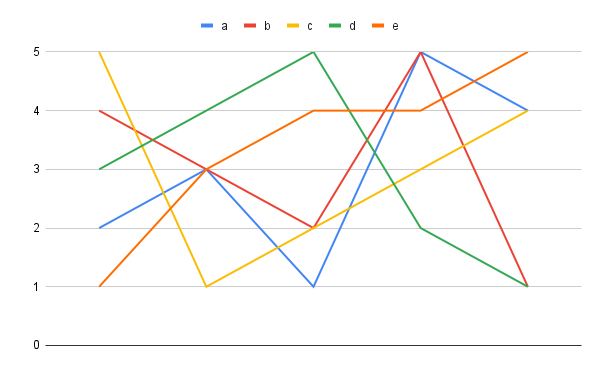
\includegraphics[width=0.5\textwidth]{2-1.png}
  \caption{図1.折れ線グラフ1}
  \label{fig:2-1} % ラベルを付けることで参照可能に
  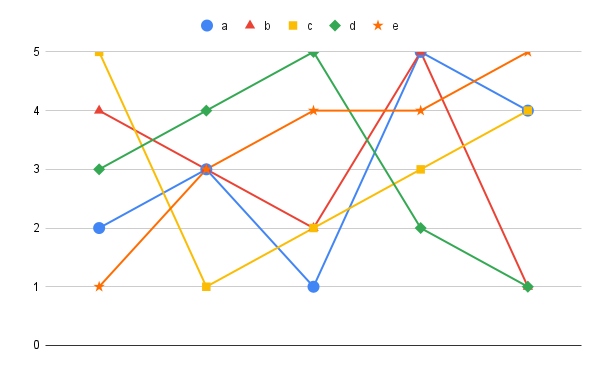
\includegraphics[width=0.5\textwidth]{2-2.png}
  \caption{図2.折れ線グラフ2}
  \label{fig:2-2} % ラベルを付けることで参照可能に
  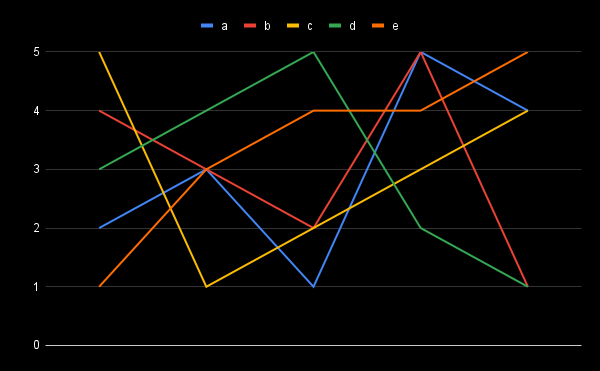
\includegraphics[width=0.5\textwidth]{2-3.png}
  \caption{図3.折れ線グラフ3}
  \label{fig:2-3} % ラベルを付けることで参照可能に
  \newpage
  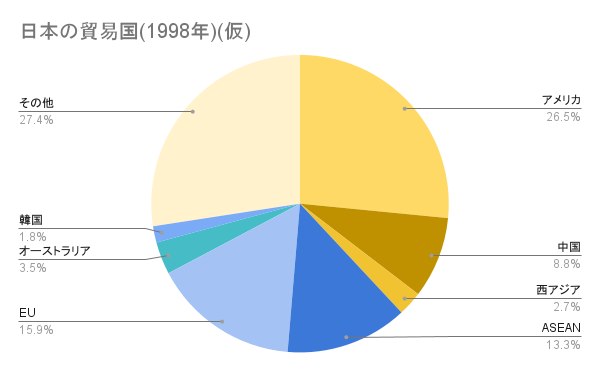
\includegraphics[width=0.5\textwidth]{2-4.png}
  \caption{図4.円グラフ1}
  \label{fig:2-4} % ラベルを付けることで参照可能に
  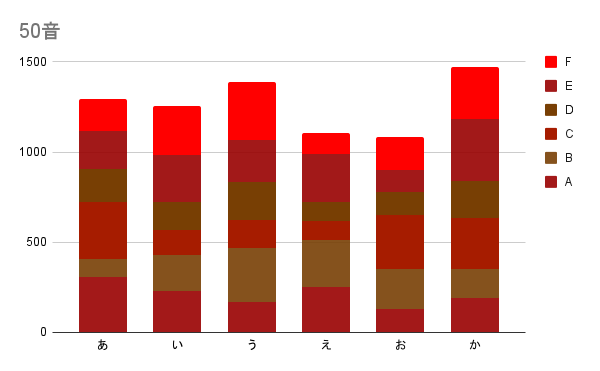
\includegraphics[width=0.5\textwidth]{2-5.png}
  \caption{図5.棒グラフ1}
  \label{fig:2-5} % ラベルを付けることで参照可能に
  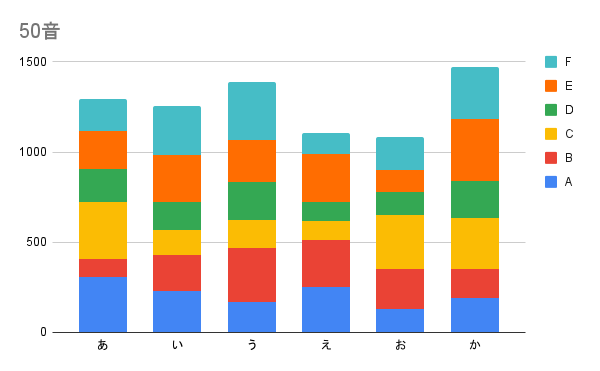
\includegraphics[width=0.5\textwidth]{2-6.png}
  \caption{図6.棒グラフ2}
  \label{fig:2-6} % ラベルを付けることで参照可能に
  \newpage
  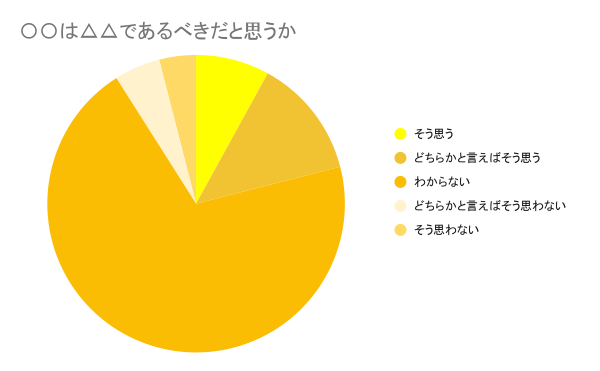
\includegraphics[width=0.5\textwidth]{2-7.png}
  \caption{図7.円グラフ2}
  \label{fig:2-7} % ラベルを付けることで参照可能に
  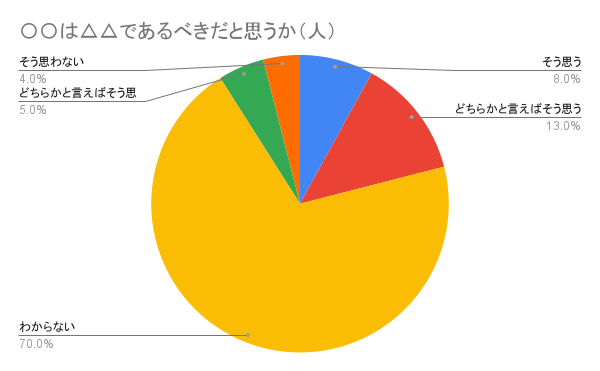
\includegraphics[width=0.5\textwidth]{2-8.png}
  \caption{図8.円グラフ3}
  \label{fig:2-8} % ラベルを付けることで参照可能に
\end{figure}
\section{北村翁}
\section{アプリケーション}
\subsection{機能概要}
 作成したウェブページには、ユーザーの利便性を考慮し、以下の主要な機能を実装した。それぞれの機能は独立しつつも相互に連携しており、効率的かつ直感的な操作が可能な仕組みを構築した。
\begin{description}
  \item[1] 画像挿入機能\\
  ユーザーが任意の画像を選択し、ウェブページ上にアップロードすることで、システムがその画像を読み込む機能を実装した。この機能では、アップロードされた画像のパスが内部で管理され、Pythonコードに引き渡されるように設計されている。これにより、画像に基づいた動的な処理を実現した。今回であれば、画像解析、色変換、加工などの処理をサーバーサイドで行い、結果をユーザーにリアルタイムで返すことが可能である。\\
  \item[2] ダウンロード機能\\
  処理が完了した画像や生成されたファイルを、ユーザーが直接デバイスにダウンロードできる機能を追加した。これにより、変換後の画像やデータを即座に利用することができる。ファイル形式は、JPEG、PNG、PDFなど、多様な形式に対応可能とした。また、ユーザーが複数の選択肢から希望する形式を選択できるようにすることで、柔軟性を向上させている。\\
  \item[3] 型選択機能\\
  ウェブページ上に、ユーザーが特定の「型」を選択できるインターフェースを用意した。この「型」によって処理内容や結果が変化する仕組みを導入している。たとえば、特定の処理パターンを選ぶと、色覚異常の種類に応じた最適な配色変換やフィルタリングが自動的に適用される。この動的な選択機能により、多様なニーズに応えるアプリケーションを実現した。\\
  \item[4] 画像変更機能\\
  「型選択機能」と連動して、画面右下に表示される画像が動的に切り替わる仕組みを実装した。この機能により、選択した型に応じた画像プレビューが即座に反映され、ユーザーは選択内容を直感的に把握できる。PC環境ではマウスカーソルを画像上に置くだけで変更内容を確認でき、スマートフォン環境では型選択時に自動的に画像が切り替わる仕様となっている。これにより、それぞれの色覚異常の型理解を手助けすることが可能となっている。
\end{description}
\writer{水島知周}
\subsection{PythonAnywhere 上でのウェブページ公開プロセス}
\begin{description}
  \item[1] 仮想環境の利用\\
  PythonAnywhere では仮想環境を構築することができ、これを活用することで特定の Python バージョンやライブラリを選択的に使用することが可能である。仮想環境を利用することで、プロジェクトごとに依存関係を適切に管理し、不要なライブラリのインストールやバージョンの競合を避けることができた。この仕組みにより、開発の効率化と安定した実行環境の確保が実現された。\\
  \item[2] 制約と適用範囲\\
  無料プランでは、CPU 時間やストレージ容量に制限があるものの、これらは小規模なウェブページを公開するには十分な性能を持っている。特に、今回のような画像処理やユーザーインタラクションを含むシンプルなウェブアプリケーションでは、これらのリソースが大きな制約となることは無かった。プロジェクト規模が拡大した場合には、有料プランへの移行も検討する余地が存在する。\\
  \item[3] ユーザビリティ\\
  PythonAnywhere は、初心者にも利用しやすいプラットフォームである。特別なサーバー設定を必要とせず、直感的なインターフェースを通じてウェブページの公開が可能である。また、インストール済みのライブラリが豊富に用意されているため、初期セットアップの時間を短縮できた。
\end{description}
\writer{小坂高義}
\section{結論}
 以上の機能を実装し、最終的には図やグラフをスマートフォンで撮影した画像を、色覚障がい者でも認識しやすい色に変換するアプリケーションを構築した。このアプリケーションは、平均2秒以内で画像変換を完了する高速な処理性能を持ち、色覚異常の種類ごとに最適化された配色を提供する。ユーザーインターフェースもわかりやすく設計されており、誰でも簡単に利用できる実用性の高いシステムとなった。
\writer{小坂高義}

\chapter{考察}
\section{得られた成果}
 本プロジェクトを通じて、色覚障がい者向けの色変換技術が、彼らの日常生活における情報認識能力の向上に寄与する可能性が高いことが示された。また、カラーユニバーサルデザインを採用することの重要性を再確認し、適切な配色の工夫が色覚障がいを持つ人々にとって視認性を大幅に向上させることを確認した。本研究では、PythonAnywhereをホスティングプラットフォームとして使用したが、これによりPythonコードを直接ウェブアプリケーションに組み込むプロセスの手軽さが実感された。同プラットフォームは、特に小規模プロジェクトや個人開発に適しており、初心者でも比較的短期間でアプリケーションの構築と公開が可能であることが分かった。一方で、無料プランにはリソース制限があり、ストレージ容量やCPU使用時間に制約があるため、大規模プロジェクトでは有料プランへの移行や他のホスティングプラットフォームの活用を検討する必要性が浮き彫りとなった。これらの点を踏まえ、開発環境の選定はプロジェクト規模や要件に応じて柔軟に対応することが求められる。また、今回の取り組みを通じて、色覚補助技術がより広範な用途に応用可能であることも確認でき、教育分野や公共施設での導入にも期待が寄せられる。
\writer{佐々木工}

\section{妥当性}
 本研究で得られた結果は、カラーユニバーサルデザインの原則に基づく配色変換が色覚障がい者の視認性向上に効果的であることを示している。しかし、候補の一つとして検討されたカメラを用いたリアルタイム色変換アプリケーションとの比較では、今回のシステムが全ての状況において最適な選択肢とは言い難い。特に、リアルタイム性が求められる場面や動的な環境においては、本プロジェクトで開発した静的なウェブアプリケーションの使用に制限がある可能性がある。また、結果の妥当性を評価する際には、利用者視点での実地テストが限られていたことが課題として挙げられる。色覚障がい者を対象としたさらなるユーザビリティテストを実施することで、開発したシステムの有用性をより正確に評価できると考えられる。
\writer{水島知周}

\section{用いた手法の限界と改善策}
 今回採用した手法において、色覚補助のアルゴリズムは基本的な変換精度を達成したが、特に細かな色差の識別が求められる場面では限界が見られた。この問題は、使用した色変換アルゴリズムが従来型の固定的な変換ロジックに依存していたためであり、複雑な色空間における動的な変換が困難であった点が原因と考えられる。
今後の改善策としては、Lab*色空間を用いた高度な変換アルゴリズムの開発が挙げられる。このアプローチでは、ユーザーの色覚特性に応じた最適な色変換を動的に計算することが可能となる。また、深層学習を利用して個別最適化された色変換モデルを構築することで、さらに正確な補助が提供できる可能性がある。
さらに、代替テキスト生成機能についても精度向上が必要とされる。現在の技術では、色識別が困難な状況下での補足情報提供が限定的であるため、OCR(光学文字認識)技術や自然言語処理モデルを統合し、画像内の情報を即時かつ的確に伝える仕組みの構築が有望である。特に、深層学習を活用した画像認識アルゴリズムやコンテキスト認識型のテキスト生成モデルを導入することで、ユーザーエクスペリエンスをさらに向上させることが期待される。
\writer{小坂高義}

\section{今後の課題・展望}
 これらの新たなテーマの実現には、技術的なスキルの向上と、色覚障がい者を含む多様なユーザーからの継続的なフィードバックが重要である。特に、ウェアラブルデバイス向けアプリケーションの開発では、デバイスの処理能力やバッテリー消費を考慮しながら、リアルタイム処理が可能な軽量なアルゴリズムの実装が課題となる。また、教育教材の開発では、視覚的な補助だけでなく、音声や触覚による情報提供を組み合わせることで、より包括的な教材を提供できる可能性がある。さらに、公共施設やウェブサイトにおける色覚バリアフリー設計の研究では、ユーザーの視点に基づいた実証実験や調査を実施し、色使いにおける新たな基準を提案することが求められる。この分野の研究成果を社会に発信することで、色覚バリアフリーに対する理解を広め、より多くの企業や団体が取り組みを進めるきっかけを作りたい。また、プロジェクトの進展に伴い、クラウドプラットフォームを活用したデータの共有と分析も視野に入れるべきである。これにより、プロトタイプの開発から実用化に至る過程を効率的に進められるだけでなく、異なる地域や文化の色覚障がい者にも対応できるグローバルな解決策の構築が可能となる。最後に、プロジェクトメンバーの連携とコミュニケーションをより深めることで、目標達成に向けたスムーズなプロジェクト進行を実現する。チームの多様な意見を尊重しながら、新しいアイデアやアプローチを取り入れることで、色覚障がい者の支援においてさらなる進化を目指したい。これらの課題に対し、技術的な工夫や社会的な連携を通じて解決策を模索し、より多くの人々が色覚バリアフリーな社会を享受できるよう尽力することを目指す。
\writer{北村翁}

\newpage\clearpage
\vspace*{-20pt}
\addcontentsline{toc}{chapter}{参考文献}  % 目次に「参考文献」を追加
\printbibliography[segment=\therefsegment,heading=subbibliography]
